% Clément CAUMES Yassin DOUDOUH
% 09 janvier 2018
% PROJET FRACTALES IN505

% Fichier de rapport du projet FRACTALES

\documentclass[a4]{article}

\usepackage[utf8]{inputenc}
\usepackage[french]{babel}
\usepackage{graphicx}
\usepackage{hyperref}
\usepackage{listings}

\author{Clément Caumes - Yassin Doudouh}
\title{Rapport du projet Fractales}
\date{09 janvier 2018}

\begin{document}
\maketitle

\section{Introduction}

Le but du projet est de créer une application permettant de créer des fractales de Mandelbrot ainsi que celles de Julia et Fatou. 
Elles correspondent à des formes geométriques complexes. Elles se construisent selon un algorithme de suites de complexes. 
\vspace{1\baselineskip}

L'application doit pouvoir permettre à l'utilisateur de construire selon ses envies la fractale de Mandelbrot et celles de Julia et Fatou. 
Celles de Julia et Fatou nécessitent la déclaration d'un nombre complexe. L'application devra proposer 2 nombres complexes intéressants : 
$ c_1 = -0.0519 + i0.688 $ et $c_2 = -0.577 + i0.478$.
\vspace{1\baselineskip}

Lorsque l'utilisateur aura choisi d'afficher la fractale, il pourra zoomer, dezoomer ainsi que se déplacer sur l'image à l'aide des touches du clavier. 
Il pourra également changer la couleur de la fractale dont les points de celle-ci auront des couleurs différentes selon leur convergence. 
Il pourra aussi modifier la granularité du dessin de la fractale : c'est-à-dire diminuer la distance entre les pixels permettra d'avoir plus de détails sur la fractale. 
L'utilisateur pourra également modifier certains paramètres de la fractale : $z_{max}$ ainsi que le complexe (pour la fractale de Julia et Fatou). 

L'application peut également proposer à l'utilisateur de faire un enregistrement vectoriel. Cela consiste à créer un fichier SVG : un bouton \emph{Enregistrer} le permet. 
\vspace{1\baselineskip} 

\section{Modélisation des classes}

Afin de comprendre plus facilement la création et l'utilisation de nos classes : nous pouvons voir ci-dessous le diagramme UML simplifié de l'application. 
Des flèches pleines représentent les héritages entre les classes ; et les flèches creuses représentent les utilisations d'une classe dans une autre (que ce soit avec un attribut ou bien dans une méthode). 

\hspace{-4cm}
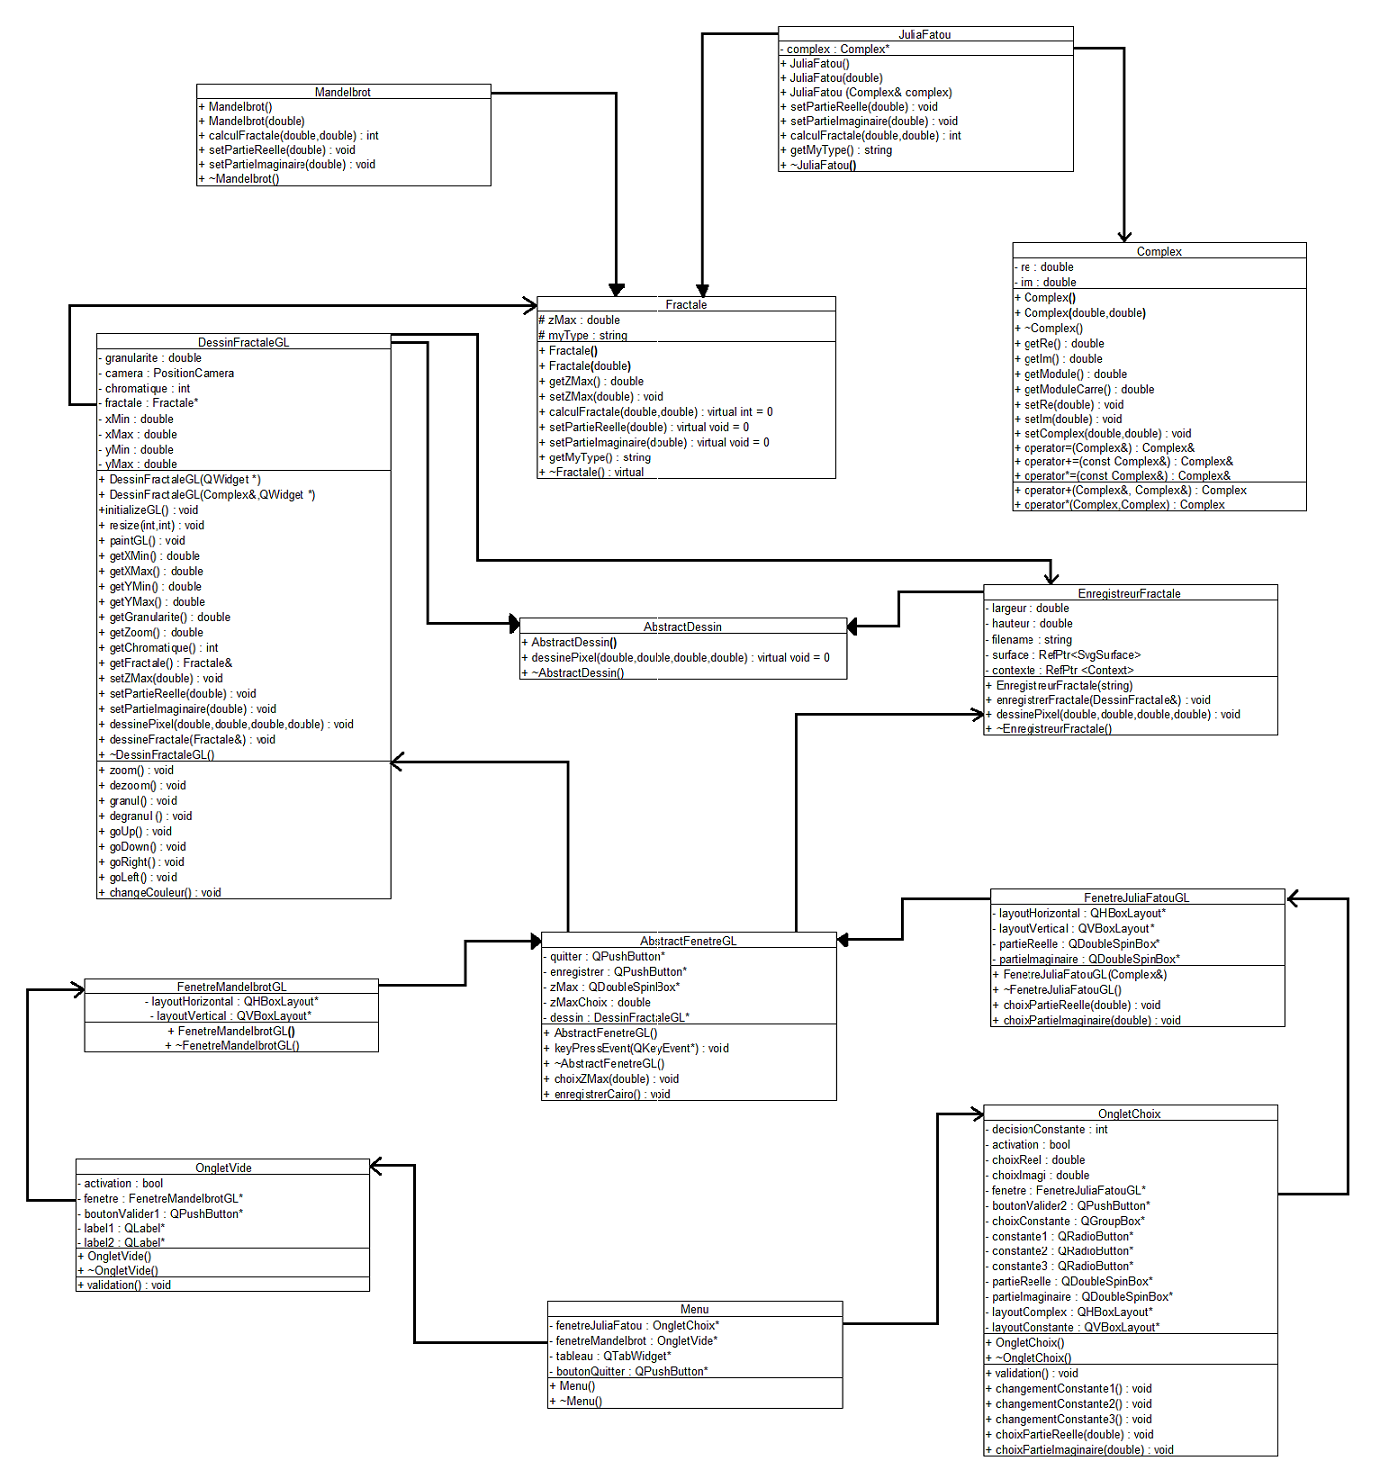
\includegraphics[height=20cm]{UML.png}

\section{Description des classes}

\subsection{Complex, Fractale, Mandelbrot, JuliaFatou}

Tout d'abord, afin de pouvoir manipuler les fractales, il a fallu définir une première classe \emph{Complex} représentant un nombre complexe. 
Pour apprécier l'utilisation de ces nombres complexes, nous avons redéfini les opérateurs $=$, $+$ et $*$ afin de ne pas surcharger le code lors de calculs de complexes. 
\vspace{1\baselineskip} 

Ensuite, nous avons créé une classe abstraite \emph{Fractale} représentant une fractale en général. 
\vspace{1\baselineskip} 

Les classes \emph{Mandelbrot} et \emph{JuliaFatou} correspondent aux classes filles de \emph{Fractale}. Elles ont en commun la méthode \emph{calculFractale} qui diffère entre \emph{Mandelbrot} et \emph{JuliaFatou}. 
Dans \emph{DessinFractaleGL} (qui sera vu par la suite), en fonction de la fractale choisie, le constructeur de celui-ci ne sera pas le même. Ainsi, le constructeur de la fractale (\emph{Mandelbrot} ou \emph{JuliaFatou}) sera différent. 
C'est pour cela que le destructeur de \emph{Fractale} doit être virtuel : \emph{DessinFractaleGL} saura quel destructeur appelé. 
\vspace{1\baselineskip}

\subsection{AbstractDessin, DessinFractaleGL, EnregistreurFractale}

La classe \emph{AbstractDessin} est la classe abstraite, demandé dans l'énoncé du projet, qui permet de construire des dessins. 
Elle a une méthode virtuelle pure \emph{dessinePixel} qui varie en fonction de l'interface (OpenGL ou Cairo). 
\vspace{1\baselineskip} 

C'est pour cela que nous avons créé deux sous-classes \emph{DessinFractaleGL} pour OpenGL et \emph{EnregistreurFractale} pour Cairo. 
Chacune des deux interfaces permettent de dessiner mais ont des méthodes différentes. Pour cette raison, il a fallu redéfinir la méthode de la classe mère 
\emph{dessinePixel} afin de pouvoir dessiner dans les deux interfaces. 
\vspace{1\baselineskip} 

La classe \emph{DessinFractaleGL} correspond à un dessin dans un widget OpenGL tandis que \emph{EnregistreurFractale} de Cairo permet d'enregistrer la fractale sous un fichier SVG. 
\vspace{1\baselineskip}

\subsection{AbstractFenetreGL, FenetreMandelbrotGL, FenetreJuliaFatouGL}

Ensuite, nous avons défini une classe abstraite \emph{AbstractFenetreGL} pour pouvoir intégrer n'importe quel dessin de Fractale. Il intègre les boutons de bases tel que celui pour quitter 
ou pour enregistrer un fichier SVG. 

Pourtant, selon la fractale choisie par l'utilisateur, la fenêtre n'est pas la même : en effet, la manipulation du nombre complexe est nécessaire dans le cas de Julia et Fatou. 
C'est pour cela que nous avons créé deux sous classes filles \emph{FenetreMandelbrotGL} et \emph{FenetreJuliaFatouGL} héritant de la classe \emph {AbstractFenetreGL}. 

\subsection{Menu, OngletVide, OngletChoix}

Afin d'apprécier le choix de la fractale choisie ainsi que ses paramètres (selon celle-ci), nous avons créé une classe \emph{Menu} qui possède deux onglets : 
un onglet pour la fractale de Julia et Fatou, et un autre pour celle de Mandelbrot. 
Ces deux onglets correspondent respectivement aux classes \emph{OngletChoix} et \emph{OngletVide}.
\vspace{1\baselineskip}  

L'onglet pour la fractale Julia et Fatou possède un ensemble de choix concernant le nombre complexe. 
En effet, l'utilisateur peut choisir les deux constantes $c=-0.0519 + i0.688$ et $c=-0.577 + i0.478$, mais aussi un nombre complexe "personnel". 
\vspace{1\baselineskip}

Dans les deux onglets, l'utilisateur pourra voir le résultat du dessin de la fractale choisie en cliquant sur \emph{Valider}.

\section{Description des principales méthodes}

La méthode redéfinie \emph{calculFractale} de \emph{Mandelbrot} et celle de \emph{JuliaFatou} correspond au calcul d'un point de l'image qui va contenir la fractale. 
On calcule ici le nombre d'itérations pour le point $(x,y)$. 
Dans le cas de \emph{Mandelbrot}, $c$ correspond au point du complexe. Tandis que dans \emph{JuliaFatou}, cela correspond à la constante complexe que l'utilisateur a choisi. 
Si la suite diverge alors on renvoie le nombre d'itérations. 
Sinon, la convergence correspondra à un point de la fractale et renverra \emph{FRACTALE}. 
Ainsi, si \emph{calculFractale} renvoie \emph{FRACTALE}, un point noir sera dessiné en $(x,y)$, sinon le nombre d'itérations sera utilisé pour dessiner l'extérieur de la fractale en couleur (selon sa divergence). 

\begin{lstlisting}[language=c++]
int Mandelbrot::calculFractale(double x,double y){
  int iterations;
  Complex c, z;
  c.setComplex(x,y);
  z.setComplex(0,0);
  iterations=0;
  while(iterations<ITERATIONS_MAX){
    if(z.getModuleCarre()>(zMax*zMax)){ 
      return iterations;
    }
	z*=z;
	z+=c;
	iterations++;
  }
  return FRACTALE;
}
\end{lstlisting}

\begin{lstlisting}[language=c++]
int JuliaFatou::calculFractale(double x,double y){
  int iterations=0;
  Complex z;
  Complex c(this->complex->getRe(),this->complex->getIm());
  z.setComplex(x,y);
  while(iterations<ITERATIONS_MAX){
    if(z.getModuleCarre()>(zMax*zMax)){
      return iterations;
    }
    z*=z;
    z+=c;
    iterations++;
  }
  return FRACTALE;
}
\end{lstlisting}

La méthode \emph{dessineFractale} suit l'algorithme suivant :
Pour chaque point de l'image, en itérant à chaque fois avec la granularité, on calcule le nombre d'itérations de la fractale et on dessine chaque point en fonction du résultat de leur calcul. 
Avec OpenGL, les couleurs RGB se situent entre 0 et 1. C'est pour cela que l'on divise le calcul des points de l'image par \emph{ITERATIONS\_MAX}. 
Si le calcul renvoie \emph{FRACTALE}, on dessine un point noir. Sinon, en fonction de la couleur choisie, on décide de celle-ci selon le nombre d'itérations.  

\begin{lstlisting}[language=c++]
void DessinFractaleGL::dessineFractale(Fractale& f){
  double x,y;
  double test;
  double PointFractale=(double)FRACTALE/(double)ITERATIONS_MAX;
  glBegin(GL_POINTS);
  for(x=xMin;x<xMax;x=x+(this->granularite)){
    for(y=yMin;y<yMax;y=y+(this->granularite)){ 
      test=(double)f.calculFractale(x,y)/ITERATIONS_MAX; 
      if(test==PointFractale){ 
        dessinePixel(x,y,0.0f,0.0f,0.0f);
      }
      else{
        if(this->chromatique!=MONOCHROMATIQUE){ 
          if(this->chromatique==COULEUR1)dessinePixel(x,y,
          fmod((test+test),1.0),fmod((test*test),1.0),
          fmod((test/test),1.0));
          else if (this->chromatique==COULEUR2) [...];
          else if (this->chromatique==COULEUR3) [...];
          else if (this->chromatique==COULEUR4) [...];
          else if (this->chromatique==COULEUR5) [...];
          else if (this->chromatique==COULEUR6) [...];
        }
	  }
    }
  }
  glEnd();
}
\end{lstlisting}

La méthode \emph{enregistrerFractale} correspond à la construction de la fractale. 
Tout d'abord, on calcule la taille de l'image SVG à l'aide de la granularité. 
Ensuite, on crée un \emph{SvgSurface} pour ouvrir le futur fichier et un \emph{Context} afin de pouvoir dessiner dedans. 
Enfin, en itérant sur chaque pixel de l'image, nous allons dessiner un point noir si le calcul de fractale renvoie \emph{FRACTALE}. 
Pour l'enregistrement Cairo, nous avons choisi de dessiner en noir et blanc la fractale (même lorsque l'utilisateur choisit une fractale en couleur avec OpenGL)
pour des raisons de performances : en effet, plus de pixels seront dessinés et cela rend l'ouverture du fichier très longue. 

\begin{lstlisting}[language=c++]
void EnregistreurFractale::enregistrerFractale(DessinFractaleGL& dessin){
  double calculTaille=((dessin.getXMax()-dessin.getXMin())/
  dessin.getGranularite());
  this->largeur=calculTaille;
  this->hauteur=calculTaille;
  this->surface = SvgSurface::create(this->filename,this->largeur, 
  this->hauteur);
  this->contexte = Context::create(surface);
  contexte->set_source_rgb(0, 0, 0); //dessin de couleur noire
  contexte->set_line_width(1); //taille d'un pixel
  double compteurX=dessin.getXMin(); 
  double compteurY=dessin.getYMax();	
  double x,y;
  int test;
  for(x=0;x<(this->largeur); x=x+0.5){ 
    compteurY=dessin.getYMax();
    for(y=0;y<(this->hauteur);y=y+0.5){
      test=dessin.getFractale().calculFractale(compteurX,
      compteurY);
      if(test==FRACTALE) dessinePixel(x,y,0,0,0);
      compteurY-=dessin.getGranularite(); 
	}
	compteurX+=dessin.getGranularite();
  }
  contexte->stroke(); //pour finaliser le dessin d'un pixel
}
\end{lstlisting}

La méthode \emph{enregistrerCairo} permet d'enregistrer vectoriellement la fractale. 
Si la distance entre les pixels n'est pas trop faible, l'application va lancer cet enregistrement. Sinon, un message sera lancé pour des raisons de performances. 
Afin d'enregistrer un fichier svg à chaque fois que l'utilisateur le veut, il a fallu choisir un nom de fichier adéquat pour ne pas supprimer un autre enregistrement. 
C'est pour cela que cette méthode va calculer le temps et ainsi créer un nouveau fichier comme \emph{"save/MandelbrotHHMMSS.svg"}. A partir de ce nouveau nom de fichier, 
nous allons pouvoir dessiner la fractale dans celui-ci. 

\begin{lstlisting}[language=c++]
void AbstractFenetreGL::enregistrerCairo(){
  if(this->dessin->getGranularite()>0.001){ 
    time_t t=time(NULL);
    struct tm* temps=localtime(&t);
    int hour=temps->tm_hour;
    int min=temps->tm_min;
    int sec=temps->tm_sec; 
    std::string titre = "save/"+
    (this->dessin->getFractale().getMyType());
    titre+= std::to_string(hour);
    titre+= std::to_string(min);
    titre+=std::to_string(sec);
    titre+=".svg";
    EnregistreurFractale enregistreur(titre);
    enregistreur.enregistrerFractale(*dessin);
    QMessageBox::information(this,"Cairo","Fichier cree");
  }
  else{
    QMessageBox::critical(this,"Cairo","Fichier non cree");
  }
}
\end{lstlisting}

\section{Difficultés rencontrées}

La recherche pour savoir dessiner avec OpenGL a été difficile malgré le site proposé dans l'énoncé.
En effet, les multiples installations ont été difficiles à trouver. De plus, la redéfinition des méthodes \emph{initializeGL} et \emph{resizeGL} ont été compliquées à comprendre. 
Enfin, la recherche d'informations à propos de Cairo a été compliquée à cause de l'intégration avec Qt et son installation. 

\vspace{1\baselineskip}
 
L'enseignement de Pierre Coucheney d'\href{http://www.uvsq.fr/licence-informatique-8283.kjsp?RH=FORM2}{Applications informatiques (IN202)} nous a permis de comprendre plus facilement les algorithmes 
pour dessiner les fractales de Mandelbrot, Julia et Fatou. 

\vspace{1\baselineskip}

Lorsque l'utilisateur choisit de diminuer la distance entre les pixels (manipulation de la granularité de la fractale) afin de voir plus de détails, et qu'il choisit d'enregistrer avec Cairo celle-ci : 
l'ouverture de ce fichier SVG la rend impossible en raison de sa taille (parfois plus d'une centaine de MegaByte). 
Pour préserver les performances de l'application, nous avons choisi de mettre une limite pour la granularité ainsi que pour l'enregistrement vectoriel. 

\vspace{1\baselineskip}

\section{Bibliographie}

Pour apprendre à utiliser la librairie graphique \emph{Qt}, nous avons utilisé le tutoriel \emph{OpenClassroom} suivant : 
\vspace{0\baselineskip}  

\url{https://openclassrooms.com/courses/programmez-avec-le-langage-c/introduction-a-qt}.
\vspace{1\baselineskip}

Pour comprendre l'utilisation de \emph{OpenGL} et son intégration à \emph{Qt}, le tutoriel proposé dans le sujet correspond à \url{http://www.digitalfanatics.org/projects/qt_tutorial/fr/chapter14.html}.
\vspace{1\baselineskip}

Après de multiples recherches pour comprendre comment effectuer un enregistrement vectoriel en utilisant \emph{Cairo}, nous avons trouvé la solution grâce aux sites suivants : 
\vspace{0\baselineskip}  
\begin{itemize}
\item \url{https://fr.wikipedia.org/wiki/Scalable_Vector_Graphics}
\item \url{https://www.cairographics.org}
\item \url{http://zetcode.com/gfx/cairo/cairobackends/}
\end{itemize}

\end{document}
